\section{SEP Prototype}~\label{sec:prototype}

With the purpose of demonstrating the feasibility of a serverless edge platform, we assembled and extended state-of-art open source tools to materialize the proposed architecture for different application scenarios.
%, evaluating it in different aspects. 
%Figure~\ref{fig:Serverless_Edge_Platform_Overview} presets an overview of the SEP prototype containing all the proposed services. In addition to the services discussed in Section~\ref{sec:SEP}, it includes a \textit{Reverse Proxy}, which is responsible for proxying external HTTP/WebSocket requests to internal platform services.

\begin{figure}[tbp]
	\centering
	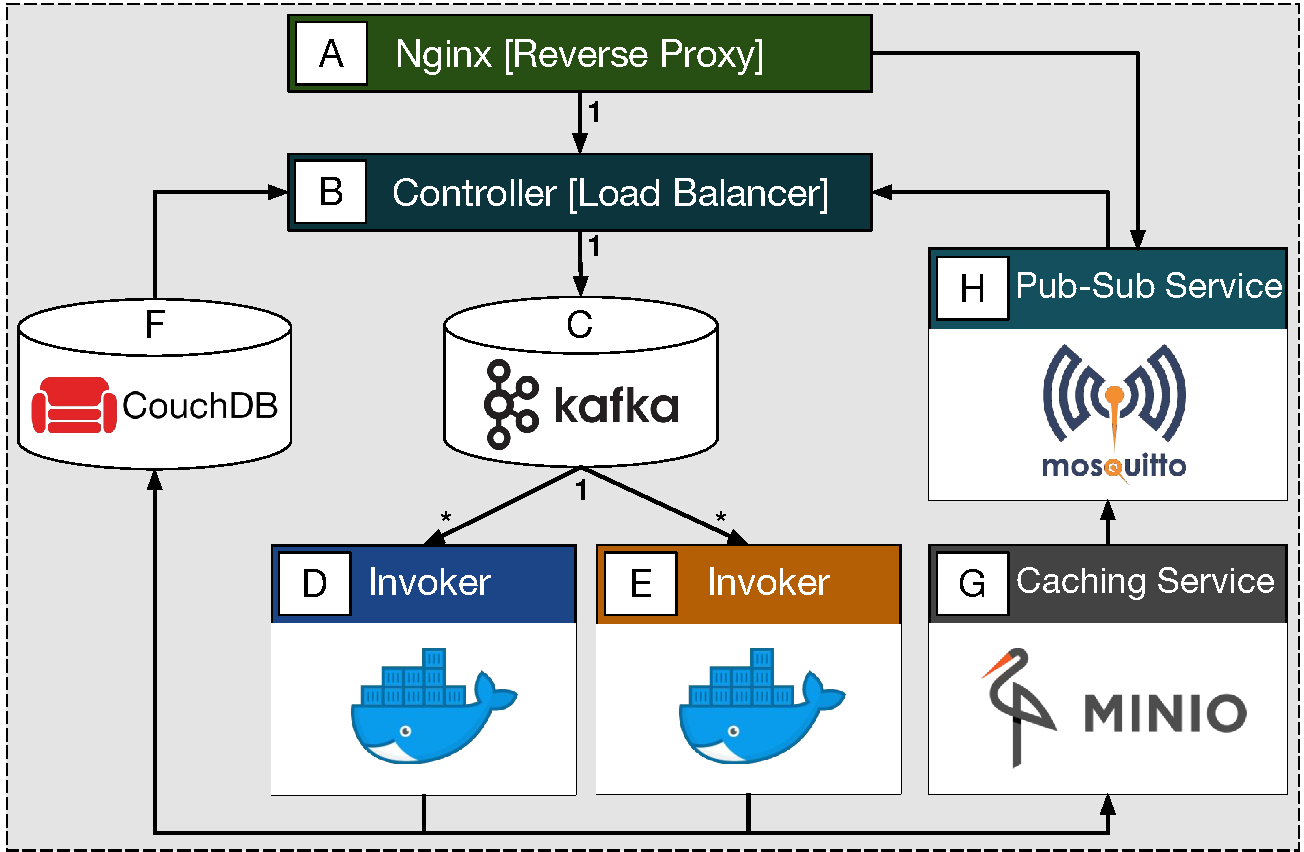
\includegraphics[width=1\linewidth]{Figs/Serverless_Edge_Platform_Prototype.pdf}
	\caption{Overview of the SEP prototype comprising all tools and services}
	\label{fig:Serverless_Edge_Platform_Overview}
\end{figure}

\subsection{Latency-Sensitive FaaS}

OpenWhisk~\cite{OpenWhisk} is a state-of-art tool implementing the FaaS model. Originally developed by IBM, it is now an open source project incubated by Apache. It is also the most mature open source FaaS tool available. OpenWhisk is the central component in the proposed SEP architecture, 
%as it takes care of the dynamic creation and termination of containerized environments. More precisely, 
as it takes of orchestrating the creation of Docker containers~\footnote{The tool recently added support other container engines} with a specific runtime (e.g., a NodeJS, python, or Java) supporting the execution of stateless functions.

%upon the activation of actions --- a stateless function written in one of the many languages supported by the tool.

%OpenWhisk is implemented as an event-driven platform. 
In OpenWhisk, functions are activated by rules associated with triggers, which in turn are mapped to internal and external events, including HTTP requests. The tool does not provide support for the WebSocket protocol. Coherently with what has been discussed in Section~\ref{sec:SEP_MCO}, we have extended OpenWhisk to enable a more efficient communication between SEPs and edge devices hosting real-time and interactive applications.  

OpenWhisk naively supports action sequences, which allow the definition of a sequential function execution flow. Our prototype exploits this feature for the definition of the \textit{workflow service} discussed in Section~\ref{sec:SEP_MCO}.

For the materialization of a SEP caching service discussed in Section~\ref{sec:SEP_MCO}, we adopted \textit{Minio}, an open source and lightweight object storage tool already part of OpenWhisk stack. Minio is compatible with \textit{AWS S3} --- a state-of-art object storage service --- and features native integration with different types of notification systems. Moreover, it features an API for managing objects. These characteristics are particularly important in the context of a SEP platform, as object events (e.g., creation, update) can trigger the execution of functions, whereas functions can access access objects through API calls. 

%an event-driven serverless architecture

%a prototype of the caching service discussed in ~\ref{sec:SEP_MCO} was implemented as a separated module in Python language. Figure~\ref{fig:SEP_Low_Latency_FaaS} presents the resulting platform architecture.

%existing containers and an \textit{Invoker} responsible for the creation and termination of containers. 

\subsection{Opportunistic FaaS}



OpenWhisk lacks support for the dynamic placement of functions based on latency requirements and other criteria. Nonetheless, it features a \textit{Load Balancer} that decides, among distributed pools of containers, where to place requests. Each pool is interfaced and managed by an \textit{Invoker} component. Invokers notify their health status with periodic heartbeats; they communicate with the \textit{Load Balancer} through messages buffered and persisted by \textit{Apache Kafka}, a high-throughput, distributed, publish-subscribe messaging system.

%an implementation of the \textit{Actor Model} featuring reliable queues.


For evaluation purposes, our SEP prototype extends OpenWhisk's native \textit{Load Balancer} to decide among edge and cloud-based execution of hosted functions. For this, the SEP \textit{Load Balancer} is aware of two invokers: a local one, and another hosted by a second node mimicking a cloud deployment. Our extension consists of two modifications: i) the initialization of an external \textit{Invoker} referencing the SEP \textit{Load Balancer}; and 2) the prioritization of the local Invoker whenever the CPU or memory load at the SEP is below 90\%. 

The prototyping of a \textit{Centralized Orchestrator} required modifications from the \textit{Invoker} side. More precisely, the activation of a given function now takes as parameter the maximum number of runtime instances a given function can have --- as decided by the \textit{Centralized Orchestrator}. If this limited is achieved, the function activation fails and the original request is put back into the \textit{Load Balancer} queue. As the response time decreases, requests are diverged to the cloud platform. Figure~\ref{fig:SEP_Placement} illustrates these components behavior.


%The evaluation of more sophisticated orchestration strategies is out of the scope of this work. 

%Contrasting with real-time FaaS, we further extended OpenWhisk's Load Balancer with scheduling capabilities. The idea is to take different latency requirements into account and prioritize those with more strict deadlines. For this, requests arriving at the SEP's Controller are sorted by means of a \textit{deadline first} algorithm before been distributed by the Load Balancer.

\subsection{Pub-Sub Service}

%Among the stack of technology composing OpenWhisk lies \textit{Kafka}, a high-throughput, distributed, publish-subscribe messaging system. 

The need for a publish-subscribe notification service is addressed with the adoption of \textit{Mosquitto}, an open source MQTT implementation largely adopted by IoT practitioners. %MQTT is the standard protocol for IoT machine-to-machine communication. 
Among its features, the Mosquitto Broker enables topic bridging and remapping. The former allows two or more brokers to become publish/subscribers of each other, so that messages published to one broker are propagated. In turn, topic renaming allows the definition of prefixes to the topics propagated from/to other brokers. The platform prototype exploit these features to allow the propagation of events from/to surrogate SEPs, as discussed in Section~\ref{sec:SEP_RTEC}. Figure~\ref{} illustrates the resulting architecture.

\subsection{Stateful Services}

To address the need of stateful services, we have enabled stateful application partitions to run in a similar environment from stateless functions by extending OpenWhisk's Invoker. In contrast with stateless functions --- which can be executed by any of the existing containers hosting its runtime environment --- stateful services are identified by a token and mapped to one specific container upon its setup at the beginning of a session. 

Every invocation to the stateful service is delegated to the corresponding container by means of an \textit{update} command. This additional command specifies the application logic to be performed along with any parameters from the original request. The resulting mechanism enables state to be consistently evolved at each invocation from one or distinct clients within the same session. Figure~\ref{} illustrates the stateful service life-cycle.

\subsection{Reverse Proxy}

Last but not least, SEPs should interface with the external world by means of a reverse proxy. Its role is to map external requests (e.g., HTTP, WebSocket) to internal services (e.g., FaaS, publish-subscribe system, etc). 

Nginx is a state-of-art tool open source tool featuring, among others, a reverse proxy. Similarly to Apache, it allows the specification of endpoints that are mapped to internal applications. Due to its maturity and popularity, we adopted Nginx as the reverse proxy in our SEP prototype. This tool is also naively integrated with OpenWhisk.

%\subsection{SEP Product Line}

%TODO: contextualize the paragraph below
%Figure~\ref{} represents the serverless edge platform as a software product line~\cite{} with product variants targeting different types of edge infrastructure and application scenarios.
